% Figure 5.10: Development Action Recommender (70-20-10)
% Compile with: pdflatex fig_5_10_action_recommender.tex

\documentclass[border=10pt]{standalone}
\usepackage{tikz}
\usetikzlibrary{shapes.geometric, arrows.meta, positioning}
\usepackage{xcolor}

% Professional academic color palette
\definecolor{layer1}{RGB}{70, 130, 180}        % Steel blue
\definecolor{layer2}{RGB}{100, 149, 237}       % Cornflower blue
\definecolor{accentteal}{RGB}{119, 176, 166}   % Muted teal
\definecolor{denseorange}{RGB}{222, 184, 135}  % Burlywood
\definecolor{outputpurple}{RGB}{186, 175, 201} % Lavender gray
\definecolor{inputgray}{RGB}{220, 220, 220}
\definecolor{textdark}{RGB}{33, 33, 33}

\begin{document}
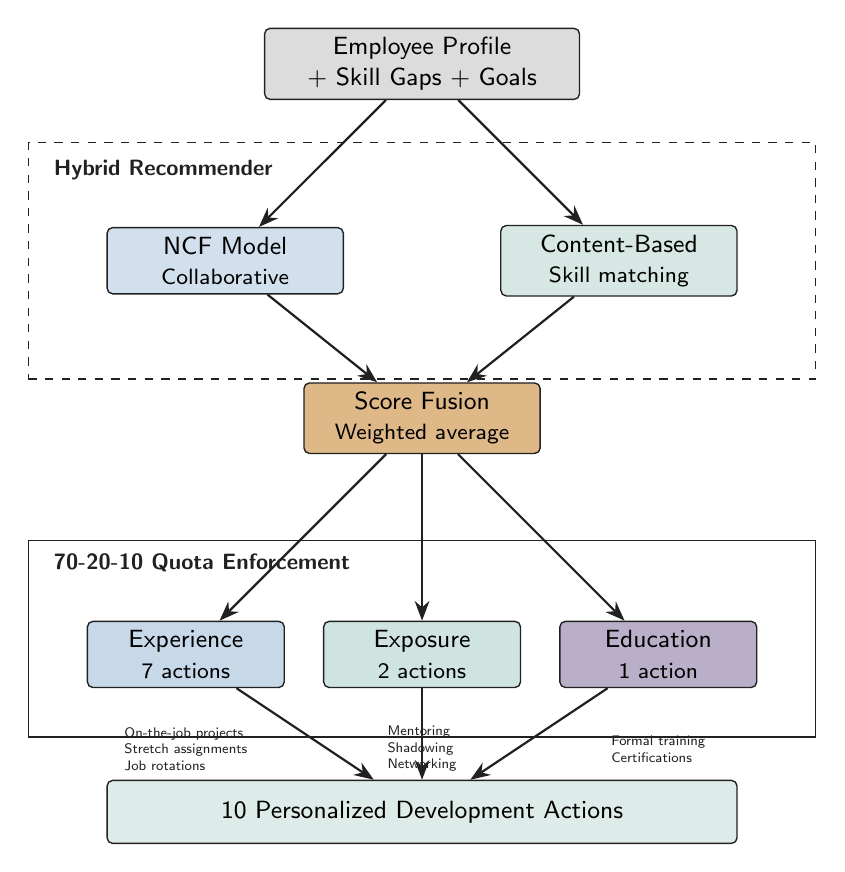
\begin{tikzpicture}[
    node distance=1cm,
    layer/.style={rectangle, draw=textdark, rounded corners=2pt, minimum width=3cm, minimum height=0.8cm, align=center, font=\small\sffamily, line width=0.5pt},
    arrow/.style={-{Stealth[length=2.5mm]}, thick, color=textdark},
]

% Input
\node[layer, fill=inputgray, minimum width=4cm] (input) at (0, 6.5) {Employee Profile\\+ Skill Gaps + Goals};

% Hybrid model
\node[rectangle, draw=textdark, dashed, minimum width=10cm, minimum height=3cm, line width=0.5pt] (hybrid) at (0, 4) {};
\node[font=\footnotesize\bfseries\sffamily, anchor=north west, color=textdark] at (-4.8, 5.4) {Hybrid Recommender};

% NCF branch
\node[layer, fill=layer1!25] (ncf) at (-2.5, 4) {NCF Model\\{\footnotesize\sffamily Collaborative}};

% Content branch
\node[layer, fill=accentteal!30] (content) at (2.5, 4) {Content-Based\\{\footnotesize\sffamily Skill matching}};

% Fusion
\node[layer, fill=denseorange, minimum width=3cm] (fusion) at (0, 2) {Score Fusion\\{\footnotesize\sffamily Weighted average}};

\draw[arrow] (input) -- (ncf);
\draw[arrow] (input) -- (content);
\draw[arrow] (ncf) -- (fusion);
\draw[arrow] (content) -- (fusion);

% 70-20-10 quota
\node[rectangle, draw=textdark, minimum width=10cm, minimum height=2.5cm, line width=0.5pt] (quota) at (0, -0.8) {};
\node[font=\footnotesize\bfseries\sffamily, anchor=north west, color=textdark] at (-4.8, 0.4) {70-20-10 Quota Enforcement};

\node[layer, fill=layer1!30, minimum width=2.5cm] (exp) at (-3, -1) {Experience\\{\footnotesize\sffamily 7 actions}};
\node[layer, fill=accentteal!35, minimum width=2.5cm] (expo) at (0, -1) {Exposure\\{\footnotesize\sffamily 2 actions}};
\node[layer, fill=outputpurple, minimum width=2.5cm] (edu) at (3, -1) {Education\\{\footnotesize\sffamily 1 action}};

\draw[arrow] (fusion) -- (exp);
\draw[arrow] (fusion) -- (expo);
\draw[arrow] (fusion) -- (edu);

% Output
\node[layer, fill=accentteal!25, minimum width=8cm] (output) at (0, -3) {10 Personalized Development Actions};

\draw[arrow] (exp) -- (output);
\draw[arrow] (expo) -- (output);
\draw[arrow] (edu) -- (output);

% Examples
\node[font=\tiny\sffamily, align=left, color=textdark] at (-3, -2.2) {On-the-job projects\\Stretch assignments\\Job rotations};
\node[font=\tiny\sffamily, align=left, color=textdark] at (0, -2.2) {Mentoring\\Shadowing\\Networking};
\node[font=\tiny\sffamily, align=left, color=textdark] at (3, -2.2) {Formal training\\Certifications};

\end{tikzpicture}
\end{document}
